\subsection{域中的整除关系}

这里我们将定义某些在代数中起重要作用的序群。通常用于这些群的记号是乘法的；因此，将先前以加法记号获得的结果应用于这些群，需要先转换为乘法记号——这对读者来说应该没有困难。在本节中，字母 A 将表示一个整环，K 表示其分式域（I，第 116 页）。

在乘法群 \(\mathbf{K}^*\) ——即 \(\mathbf{K}\) 的非零元素所成的群——中，集合 \(\mathbf{P}\) （ \(\mathbf{A}\) 的非零元素的集合）在乘法下封闭，因为 \(\mathbf{A}\) 是一个环。因此它在 \(\mathbf{K}^*\) 上通过 \(x^{-1}y\in \mathbf{P}\) 定义了一个预序关系，即“存在 \(z\in \mathbf{P}\) 使得 \(y = zx\) ”，它使 \(\mathbf{K}^*\) 成为一个（写成乘法形式的）预序群（VI，第3页，命题3）。把关于 \(\mathbf{A}\) 的元素的术语（I，第97页）推广到 \(\mathbf{K}^*\) ，关系 \(x^{-1}y\in \mathbf{P}\) 也可以表述为： \(x\) 整除 \(y\) ，或 \(x\) 是 \(y\) 的因子，或 \(y\) 是 \(x\) 的倍元（相对于环 \(\mathbf{A}\) ）；我们把关系 \(x^{-1}y\in \mathbf{P}\) 称为 \(\mathbf{K}^*\) 中相对于环 \(\mathbf{A}\) 的整除关系。关系“ \(x\) 整除 \(y\) ”记作 \(x|y\) ，其否定记作 \(x\nmid y\) 。 \(\mathbf{P}\) 的元素无非是 1 的倍元。

注记. --- 1) \(\mathbf{K}^*\) 中的整除关系本质性地依赖于所考虑的特定环 \(\mathbf{A}\) 。若 \(\mathbf{A} = \mathbf{K}\) ，我们得到“平凡”关系，在其下 \(x \mid y\) 对每一对元素 \((x, y)\) （它们属于 \(\mathbf{K}^*\) ）成立。设 \(p\) 与 \(q\) 为素数；有理数 \(r/s\) ，其分母不是 \(p\) （相应地， \(q\) ）的倍数，构成一个子环 \(\mathbf{Z}_{(p)}\) （相应地， \(\mathbf{Z}_{(q)}\) ），它是 \(\mathbf{Q}\) 的子环； \(\mathbf{Q}^*\) 中相对于这两个环的整除关系是不同的：若 \(p \neq q\) ，则数 \(p/q\) 在一个关系下是 1 的倍元而在另一个关系下不是。

\begin{enumerate}
\def\labelenumi{\arabic{enumi})}
\setcounter{enumi}{1}
\tightlist
\item
  我们有时会把关系 \(x \mid y\) 的定义推广到 \(K\) 的元素对（而不只是 \(K^*\) 的），该关系理解为“存在 \(z \in A\) 使得 \(y = zx\) ”；于是 \(x \mid 0\) 对所有 \(x \in K\) 成立。这使我们能够不加限制地陈述以下结果：若 \(x \mid y\) 且 \(x \mid z\) ，则 \(x \mid (y - z)\) ；若 \(x \mid y\) 且 \(x \nmid z\) ，则 \(x \nmid (y - z)\) 。用同样的方式，我们可以推广所有相应的术语。
\end{enumerate}

为了从整除关系得到一个序关系（第2节），我们必须过渡到 \(\mathbf{K}^*\) 关于子群 \(\mathbf{A}^*\) 的商群，这个子群由元素 \(x \in \mathbf{K}^*\) （它们满足 \(x \mid 1\) 且 \(1 \mid x\) ）组成；这些元素是 \(\mathbf{P}\) 中那样的元素，它们是 1 的因子，也就是 \(\mathbf{A}\) 的可逆元素；按语言的滥用，它们常被称为环 \(\mathbf{A}\) 的单位。商群 \(\mathbf{K}^* / \mathbf{A}^*\) 于是是一个序群。两个元素 \(x\) 与 \(y\) （属于 \(\mathbf{K}^*\) ）若属于 \(\mathbf{A}^*\) 的同一个陪集，就称为相伴元；这意味着 \(x \mid y\) 且 \(y \mid x\) 。另一方面，若 \(x\) 整除 \(y\) 而 \(y\) 不整除 \(x\) ，则我们说 \(x\) 严格整除 \(y\) ，或者说 \(x\) 是 \(y\) 的真因子，或者说 \(y\) 是 \(x\) 的真倍元。

注意 \(K^{*}/A^{*}\) 是一个滤过群，因为K是A的分式域（VI，第4页，命题4）。

说 \(K^{*}\) 的两个元素 x 与 y 是相伴的，等于说它们在 K 中有相同的倍元，这由整除关系的传递性得到。对所有 \(x \in K\) ，我们用 Ax 表示所有形如 zx 的元素组成的集合，其中 \(z \in A\) ；集合 Ax 是把 K 看作 A-模时的一个子模。把 \(x \in A\) 这一情形的术语加以推广，我们称它为域 K 相对于环 A 的主分式理想。与此相对，环 A 的理想称为整理想。

\pandocbounded{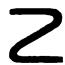
\includegraphics[keepaspectratio]{images/part002_d9406660.jpg}}

注意，若 \(\mathbf{A} \neq \mathbf{K}\) ，则一个 \(\neq \{0\}\) 的主分式理想不是把 \(\mathbf{K}\) 看作环时的理想。

主分式理想 Ax 也记作 \((x)\) 。我们将写 \(x \equiv 0 \pmod{y}\) 以表示 \(x \in Ay\) ，写 \(x \equiv x' \pmod{y}\) 以表示 \(x - x' \in Ay\) ；若 \(x \equiv x' \pmod{y}\) ，则 \(zx \equiv zx' \pmod{zy}\) 对任意 \(z \in K\) 成立。

注意，\(x \equiv x' (\bmod y)\) 并不蕴含 \(zx \equiv zx' (\bmod y)\) ，除非 \(z \in A\) 。因此在 \(\mathbf{Q}\) 中相对于 \(\mathbf{Z}\) ，有 \(4 \equiv 2 (\bmod 2)\) 但没有 \(2 \equiv 1 (\bmod 2)\) 。

关系 \(x \mid y\) 显然等价于 \((x) \supset (y)\) 。映射 \(x \mapsto (x)\) 从 \(K^*\) 映到集合 \(\mathcal{P}^*\) （由 \(\neq (0)\) 的、\(K\) 的主分式理想组成）上，从而在取商后定义了一个从 \(K^*/A^*\) 到 \(\mathcal{P}^*\) 的双射；借助这个映射把 \(K^*/A^*\) 的群结构转移到 \(\mathcal{P}^*\) 上，我们便被引导去把两个主分式理想 \((x)\) 与 \((y)\) 的乘积定义为理想 \((xy)\) ，它只依赖于 \((x)\) 与 \((y)\) 。配备了这个运算和序关系 \((x) \supset (y)\) 之后，集合 \(\mathcal{P}^*\) 构成一个序群，同构于 \(K^*/A^*\) 。按惯例，我们将通过上述映射把 \(\mathcal{P}^*\) 与 \(K^*/A^*\) 等同起来。

注意，在正整数情形下，“x 整除 y”这一关系意味着 x 小于 y，它对应于包含关系 \((x) \supset (y)\) ，其中理想 \((x)\) “大于”理想 \((y)\) 。我们可以记住这种“序反转”，例如注意到 7 的“倍数”比 91 的“更多”。

若我们把关系 \(x \mid y\) 扩展到 \(\mathbf{K}\) 的所有元素上，则此关系仍等价于 \((x) \supset (y)\) ，这里集合 \(\mathcal{P}\) 由 \(\mathbf{K}\) 的所有主分式理想组成（其中 (0) 在包含关系下是最小元素）。

如前几节一样，下文我们一般将使用加法记号。然而，与整除性有关的术语将跟在相应的加法术语之后引入，置于以记号（DIV）开头的段落中（其中约定使用本节的记号）。为方便读者，某些结果将被翻译成整除性的语言，例如命题7的翻译记作“命题7（DIV）”。

